\documentclass[draftcls,onecolumn]{IEEEtran}

%% INCLUDING THE PREAMBLE
%%%%%%%%%%%%%%%%%%%%%%%%%%%%%%%%%%%%%%%%%%%%%%%%%%%%%%%%%%%%%%%%%%%%%%%%%%%
%                                                                         %
%                                 PREAMBLE                                %
%                                                                         %
%%%%%%%%%%%%%%%%%%%%%%%%%%%%%%%%%%%%%%%%%%%%%%%%%%%%%%%%%%%%%%%%%%%%%%%%%%%

%% PACKAGES
\usepackage[]{lineno}
%\linenumbers
\usepackage[usenames,dvipsnames]{xcolor}
\usepackage{microtype}
\usepackage[obeyDraft]{todonotes}
\usepackage{fancyvrb}
\VerbatimFootnotes
\usepackage{algorithmic}

%% GRAPHICS RELATED
\usepackage{graphicx}
\usepackage[outdir=./tmp/]{epstopdf}
\graphicspath{{../images/}{./}{./tmp/}}
\DeclareGraphicsExtensions{.eps, .pdf, .jpeg, .png,}

%% CPATION SETUP
\usepackage{float}
\usepackage{caption}
\usepackage{subcaption}
\captionsetup{belowskip=12pt,aboveskip=4pt}


%% BIBLIOGRAPHY
\bibliographystyle{ieeetr}

%% UNITS
\usepackage{siunitx}

%% EQUATIONS
\usepackage{amsmath}
%\numberwithin{equation}{section}

%% HYPERLINKS
\usepackage[debug]{hyperref}

%%%%%%%%%%%%%%%%%%%%%%%%%%%%%%%%%%%%%%%%%%%%%%%%%%%%%%%%%%%%%%%%%%%%%%%%%%%
%                                                                         %
%                             Listing Setup                               %
%                                                                         %
%%%%%%%%%%%%%%%%%%%%%%%%%%%%%%%%%%%%%%%%%%%%%%%%%%%%%%%%%%%%%%%%%%%%%%%%%%%
\usepackage{listings}
\lstset{ %
    language=C++,
    basicstyle=\footnotesize\ttfamily,
    numbers=left,
    numberstyle=\tiny\color{gray},
    stepnumber=2,
    numbersep=5pt,
    backgroundcolor=\color{white},
    showspaces=false,
    showstringspaces=false,
    showtabs=false,
    frame=single,
    rulecolor=\color{black},
    tabsize=2,
    breaklines=true,
    breakatwhitespace=false,
    title=\lstname,
    keywordstyle=\color{blue},
    commentstyle=\color{OliveGreen},
    stringstyle=\color{orange}
}
\DeclareCaptionFont{white}{\color{white}}
\DeclareCaptionFormat{listing}{\colorbox[cmyk]{0.43, 0.35, 0.35, 0.01}{\parbox{\dimexpr\textwidth-2\fboxsep\relax}{#1#2#3}}}
\captionsetup[lstlisting]{format=listing,labelfont=white,textfont=white,singlelinecheck=false,margin=0pt,font={bf,footnotesize}}
%\lstnewenvironment{code}[1][]%
%{ \noindent\minipage{\linewidth}
%	\lstset{#1}
%}
%{\endminipage}
%% USER COMMANDS
\usepackage{isotope}
\newcommand{\iso}{\isotope}
\newcommand{\figurewidth}{\textwidth}
\newcommand{\micron}{$\mu$m}


\usepackage[iso,american]{isodate}
\usepackage{ctable}
%% SUBVERSION INFORMATION
\usepackage{svn-multi}
\svnidlong
{$LastChangedBy$}
{$LastChangedRevision$}
{$LastChangedDate$}
{$HeadURL$}
%%%%%%%%%%%%%%%%%%%%%%%%%%%%%%%%%%%%%%%%%%%%%%%%%%%%%%%%%%%%%%%%%%%%%%%%%%%
%                                                                         %
%                                Start of Document                        %
%                                                                         %
%%%%%%%%%%%%%%%%%%%%%%%%%%%%%%%%%%%%%%%%%%%%%%%%%%%%%%%%%%%%%%%%%%%%%%%%%%%
\begin{document}
\title{Detector Mounting Materials: PMMA Acrylic and UVT Acrylic}
\author{Matthew J. Urffer, Andrew Mabe}
\date{\today}
\maketitle

% Tables of Contents, Figures, Tables
\tableofcontents
\listoffigures
\listoftables
%%%%%%%%%%%%%%%%%%%%%%%%%%%%%%%%%%%%%%%%%%%%%%%%%%%%%%%%%%%%%%%%%%%%%%%%%%%
%                                                                         %
%                              Start of Content                           %
%                                                                         %
%%%%%%%%%%%%%%%%%%%%%%%%%%%%%%%%%%%%%%%%%%%%%%%%%%%%%%%%%%%%%%%%%%%%%%%%%%%
\section{Introduction}
Developed detector materials are often brittle and thus for repeatable characterization of the material it is often desired to cast the film unto a backing that can provide structural stability while not interfering with the measurements.
Acrylic plastic (polymethylmetharylate, PMMA) is a commonly used in fabricating light guides for plastic scintillators due to it's optical clarity and good mechanical properties and thus is a natural choice of a mounting material.
Generally the PMMA is available in two types, with or without ultra-violet (UV) absorbing materials added to the cast PMMA.
The UV absorbers are added for general purpose commercial applications and are the standard, and thus when the absorbers are omitted the material is know as UVT (ultraviolet transparent) Acrylic.
The effectiveness of the UV absorbers are shown in \autoref{fig:EJTransArcylic}.
\begin{figure}
  \centering
  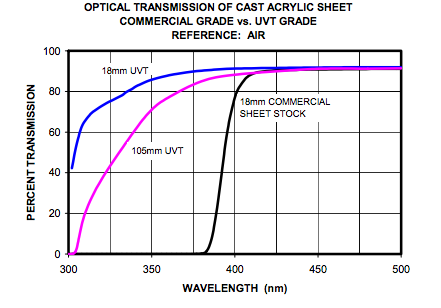
\includegraphics[width=0.5\textwidth]{EJ_ArcylicTransmission}
	\caption[Light Transmission of Eljen Acrylics (Eljen)]{Light transmission of Eljen acrylics.  The effect of the UV absorbers is shown in by the very low transmission of the commercial stock below a wavelength of \SI{375}{\nm}.}
	\label{fig:EJTransArcylic}
\end{figure}	
It was observed in repeating the neutron fraction above the gamma LLD that there was significant discrepancy between a film mounted on a thin PMMA disc and a film mounted on a thick UVT (ultra-violet transparent) acrylic disc, as shown in \autoref{tab:PSFractionRepeatMeas}.
This effect was observed for two different film thickness (\SI{25}{\um} and \SI{50}{\um}) with each film being 10\% LiF in a polystyrene matrix.
\begin{table}
	\centering
	\caption[PS Film Neutron Fraction Measurements]{Neutron Response Measurements of Polystyrene Films.  Note that the \SI{150}{\um} film has repeatable measurements, while the \SI{25}{\um} and \SI{50}{\um} do not.}
	\label{tab:PSFractionRepeatMeas}
\begin{tabular}{p{5.5cm} | m{1cm} m{1.5cm} m{1.5cm} m{2cm} m{2cm}}
\toprule
Name&Thickness&Gamma LLD \num{1E-6} (channel) & Neutron Count Rate (cps) & Neutron Count Rate Above Gamma LLD & Neutron Fraction\\
\midrule
\path{PS_LiF(10.3)_PPO(4.90)-Annealed_25um_29MayFeb2012} & 25 & 772&6.336&0.207&0.0327 \\
\path{PS_LiF(9.66)_PPO(4.58)-Annealed_26um_19Jan2012}    & 26&1100&9.742&5.073&0.5207 \\
\hline
\path{PS_LiF(9.95)_PPO(5.11)_50um_24Jan2012} &50&1352&20.686&6.453&0.3120 \\
\path{PS_LiF(10)_PPO(5)_50um_28Feb2013}		  &50&1365&12.489&0.245&0.0196 \\
\hline
\path{PS_LiF(9.88)_PPO(5)_151um_20Aug2011}	          &151&2386&53.872&0.195&0.0036 \\
\path{PS_LiF(10)_PPO(4.94)_151um_25July2011}	          &151&2385&60.615&0.189&0.0031 \\
\end{tabular}
\end{table}
It is observed from \autoref{tab:PSFractionRepeatMeas} that the gamma measurements as indicated by the MLLD are stable while the neutron count rate is not. 
It is shown in \autoref{fig:NeutronCountRateRepeat} that there is a distinct difference between the PMMA mounted and UVT mounted disc, with the PMMA mounted films having a much lower performance.

\begin{figure}
  \centering
  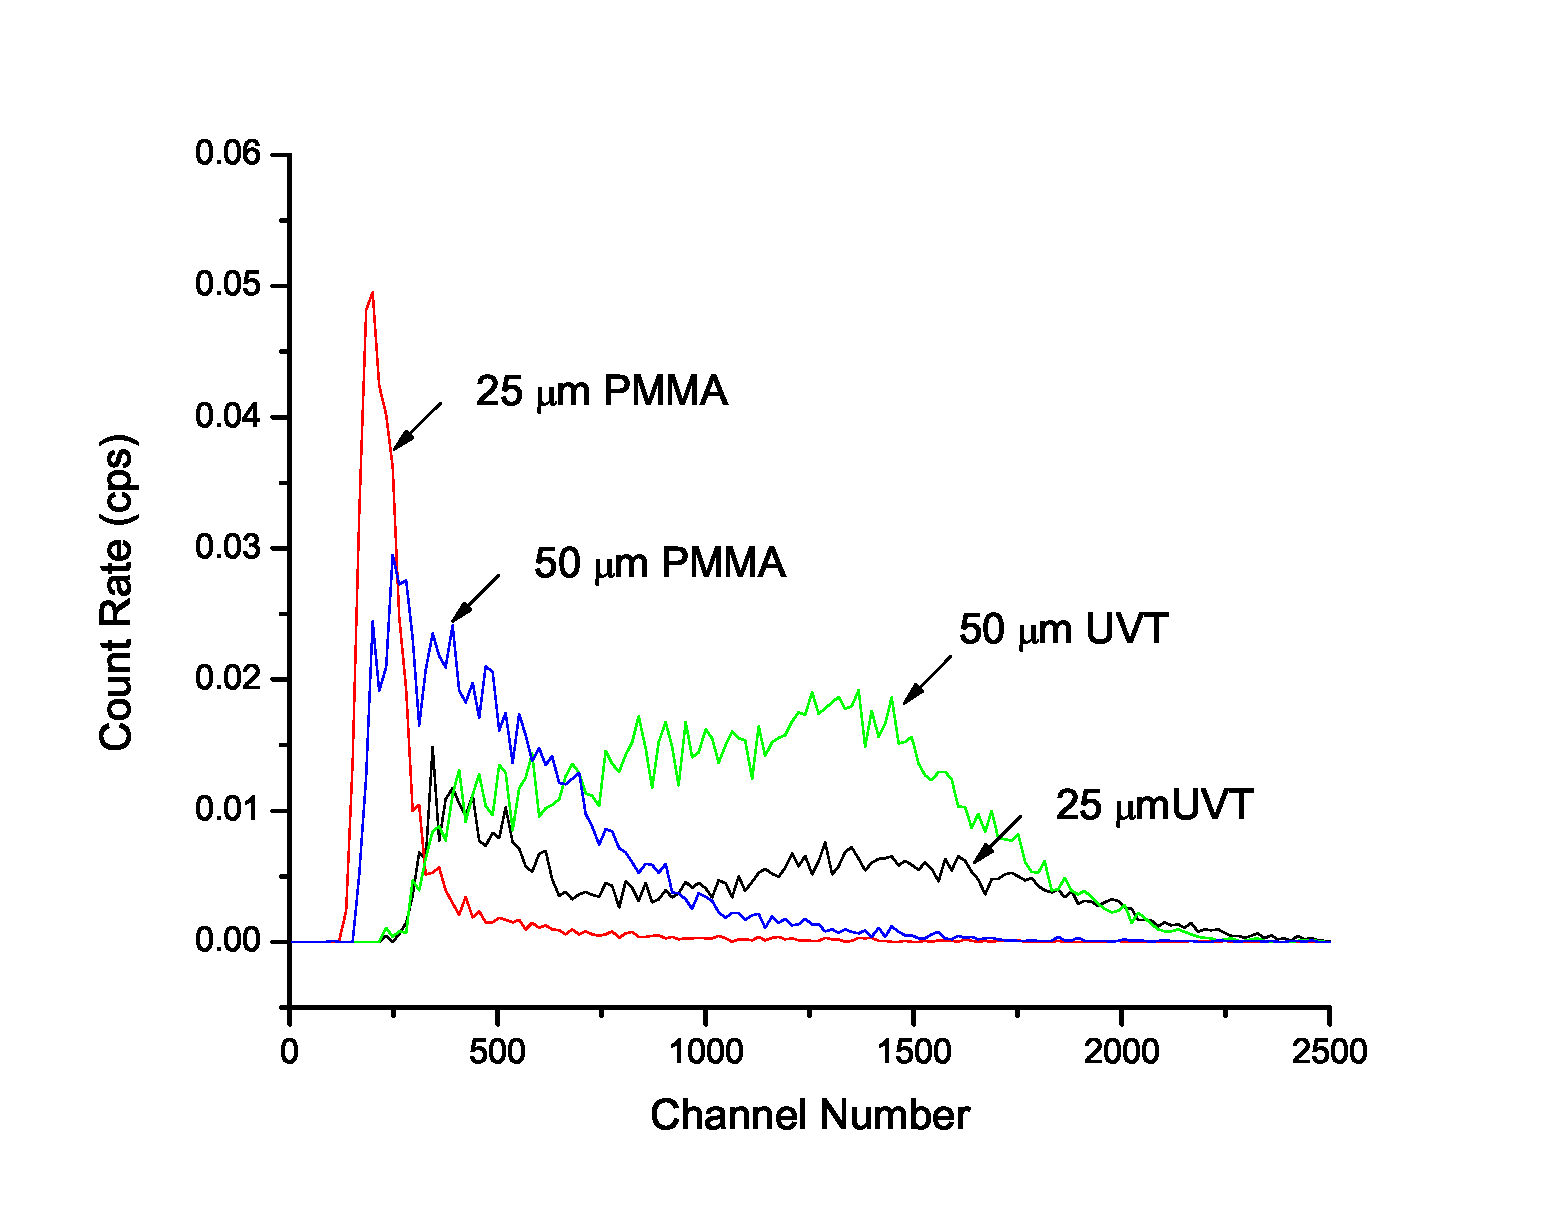
\includegraphics[width=0.7\textwidth]{UVTPMMA_CountRate}
  \caption[Neutron Spectra of UVT mounted and PMMA mounted films]{Neutron spectra of UVT mounted and PMMA mounted films.  It is evident that both UVT mounted films have the same endpoint (around 2,250 channels) while the PMMA films have a much lower neutron endpoint and a different spectra shape.}
  \label{fig:NeutronCountRateRepeat}
\end{figure}
Several different causes of this discrepancy were considered:
\begin{itemize}
  \item energy deposition by charged particles not being fully absorbed in the film (and being adversely effected by the disc),
  \item light propagation through the acrylic disc being attenuated,
  \item and adverse chemical reactions in the PMMA disc.
\end{itemize}
It was quickly ruled out that the energy deposition by the reaction products could not be responsible.
As both materials are made of the same constituents it is reasonable to expect that the reflection of electron from the disc back unto the film would be very similar.
In addition, a \iso[36]{Cl} source was placed directly on the PMT and no counts above background were absorbed, thus making it unlikely that electrons were escaping the film and interacting directly with the photo-diode on the PMT.

\section{Methods}
From the arguments made above it was determined that the cause of this discrepancy must be either light propagation in the disc, different material compositions, or additional chemistry occurring between the cast film and disc upon which it is cast.
In order to determine if it was light propagation through the films two sets of experiments were completed in which it was attempted to replicate a PMMA film as mounted on a UVT disc, and a UVT mounted film as cast on a PMMA disc.
The second (after the first failure to provide a conclusive answer) was to fabricate two more films of the same composition and batch, measuring the emission and excitation of the disc before and after, along with the scintillation properties.

\subsection{Light Transport Experiment}
The premise of these experiments is to try and replicate the same light collection geometry with the existing films.
If the back of the film is mounted in a non light reflecting geometry, the light entering the PMT must pass through the disc upon which the mounting is being tested and thus the performance of that disc can be determined.
Two different sets of experiments were preformed in order to determine if light attenuation in the film caused the degradation in performance.
The first experiment was to try and reconstruct the measurement of a PMMA disc as if it was mounted on a UVT disc, and the second was to reverse the setup and try to replicate a PMMA film as if it was cast on a UVT arcylic disc.
The geometry of the four experiments is shown in \autoref{fig:LightAttenExp}.

The experiments shown in \autoref{fig:ExpA} and \autoref{fig:ExpC} are designed to provide the performance of the film without the effects of the PMMA or UVT disc, respectively.
In the experiment shown in \autoref{fig:ExpB} it is expected under this hypothesis that the performance of the film should be dramatically reduced by the PMMA disc.
The experiment shown in \autoref{fig:ExpD} is expected to have a higher light output than the base case in \autoref{fig:ExpC}.
\begin{figure}
  \centering
  \begin{subfigure}[b]{0.45\textwidth}
    \centering
    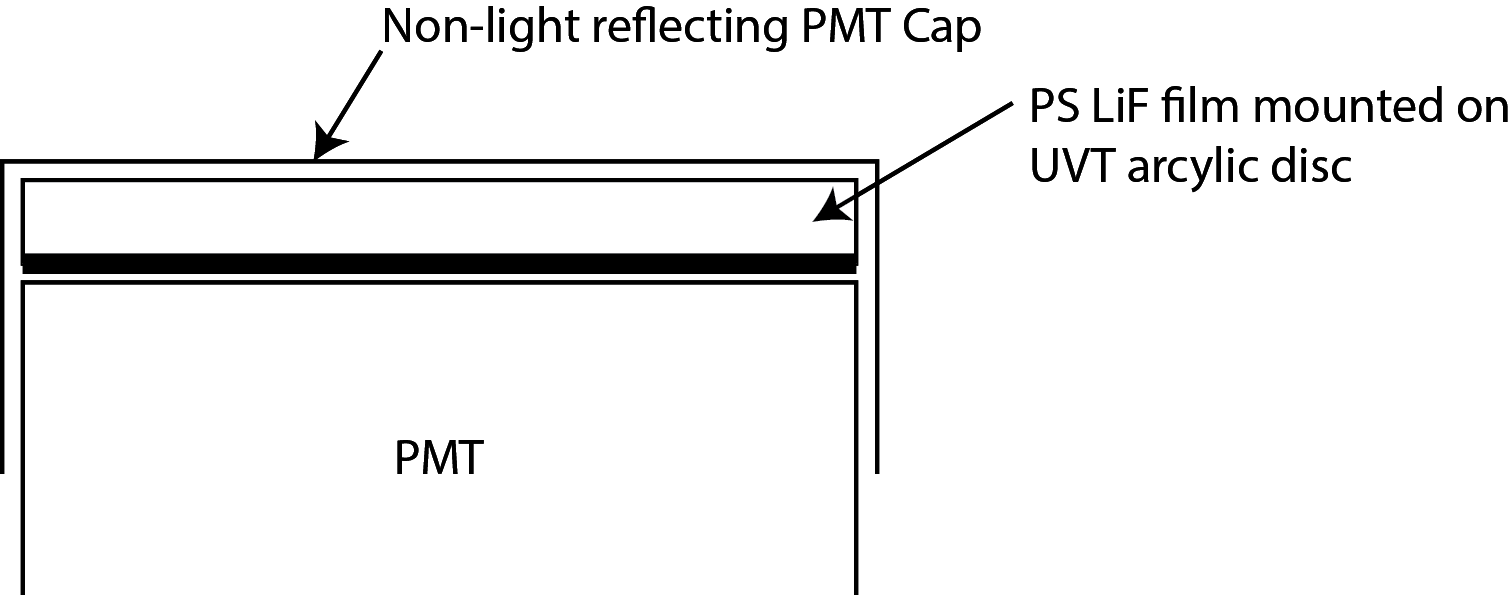
\includegraphics[width=\textwidth]{UVT_PMMA_ExperimentDesign_ExpA}
    \caption{Experiment A}
    \label{fig:ExpA}
  \end{subfigure}%
  ~
  \begin{subfigure}[b]{0.45\textwidth}
    \centering
    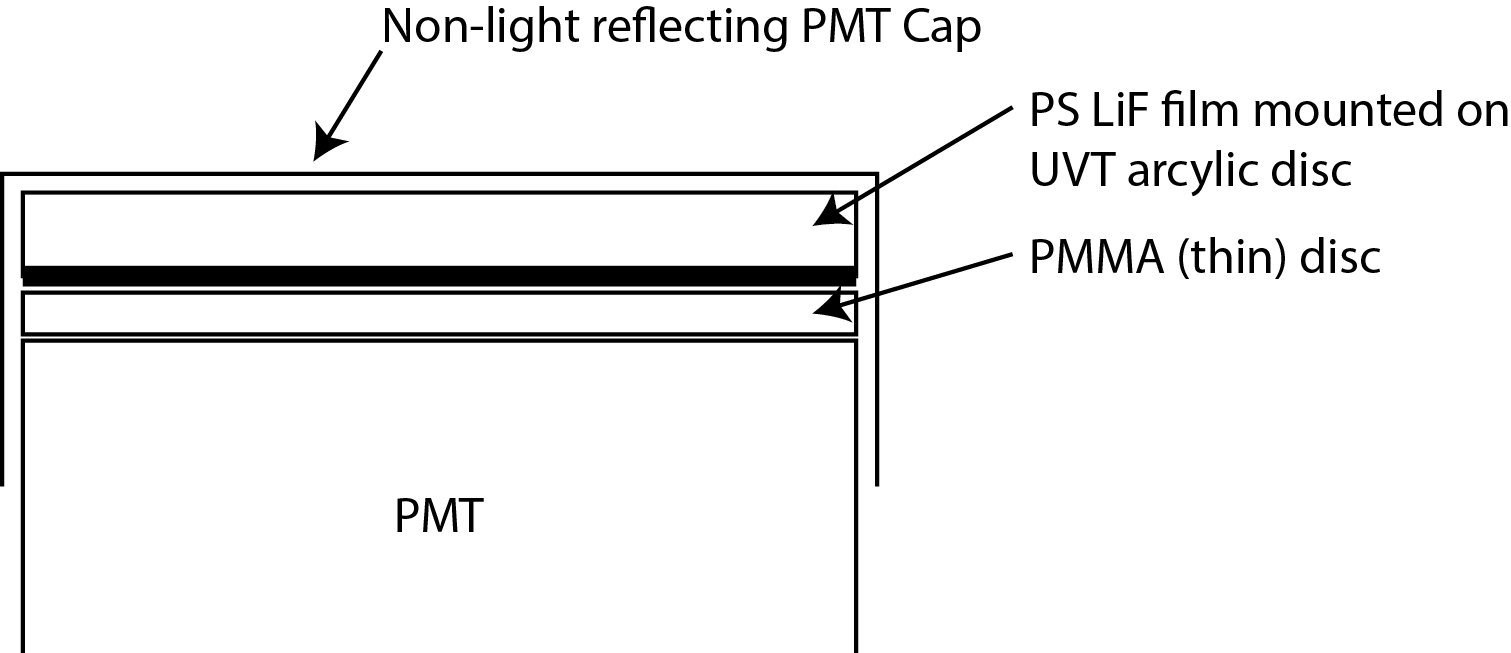
\includegraphics[width=\textwidth]{UVT_PMMA_ExperimentDesign_ExpB}
    \caption{Experiment B}
    \label{fig:ExpB}
  \end{subfigure}%
  
  \begin{subfigure}[b]{0.45\textwidth}
    \centering
    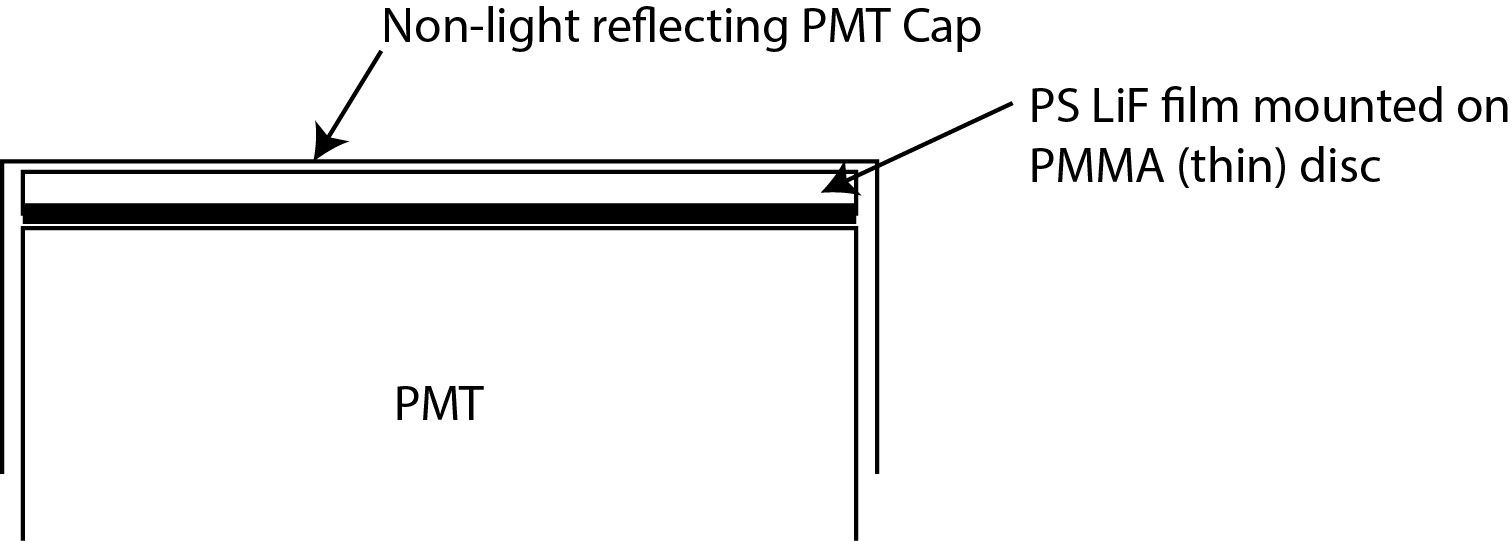
\includegraphics[width=\textwidth]{UVT_PMMA_ExperimentDesign_ExpC}
    \caption{Experiment C}
    \label{fig:ExpC}
  \end{subfigure}%
  ~
  \begin{subfigure}[b]{0.45\textwidth}
    \centering
    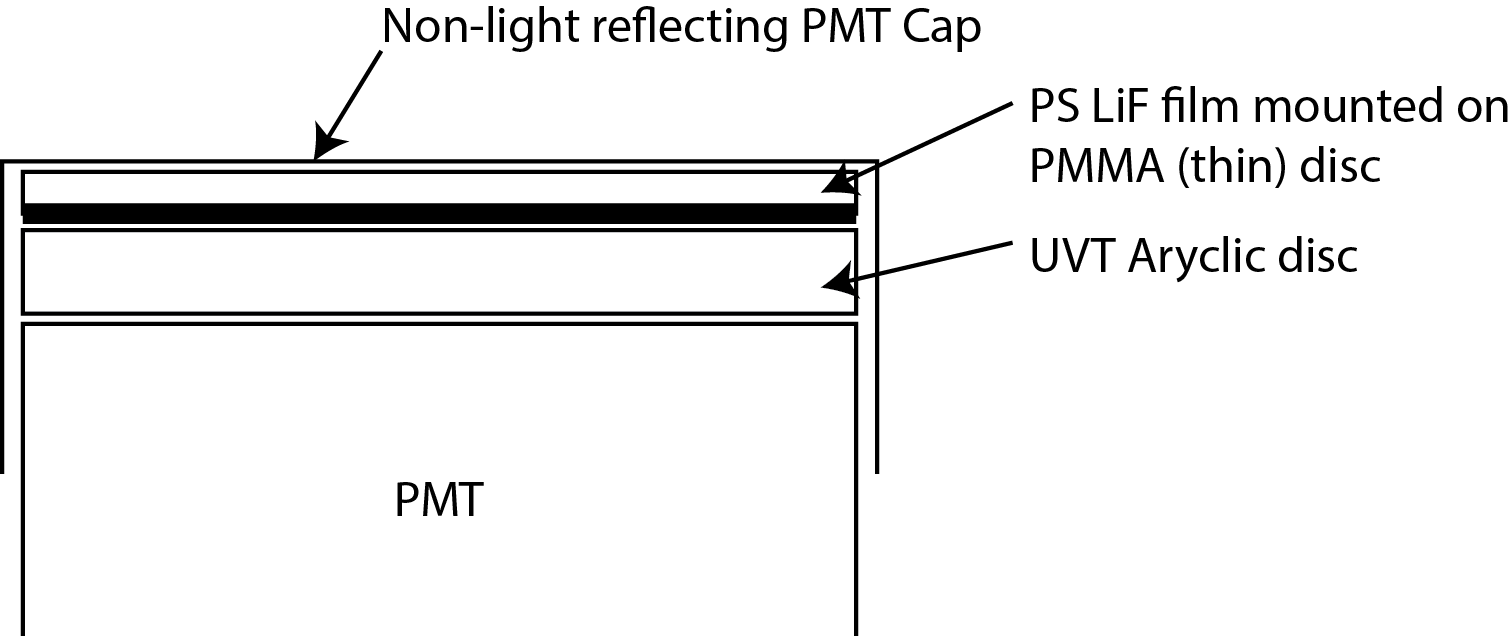
\includegraphics[width=\textwidth]{UVT_PMMA_ExperimentDesign_ExpD}
    \caption{Experiment D}
    \label{fig:ExpD}
  \end{subfigure}
  \caption[Light Attenuation Experiment Design]{Light attenuation experiment design, with the detector represented as mounted with eh solid horizontal line. It was expected that by placing the films in non-reflecting geometry that the light could be attenuated in a similar manner to being mounted on a PVT acrylic disc or a PMMA disc.}
  \label{fig:LightAttenExp}
\end{figure}
\subsection{Film Fabrication Experiment}
In order to eliminate the possiblity that poor performance of a film mounted on PMMA was due to an anomalous fabrication five additional films (85\% PS, 10\% LiF, 5\% PPO-POPOP) were fabricated from the same batch.
The light yeild of these films was then measured, as well as the determination of the neutron preformance.
One of five \SI{50}{\um} films was mounted on a \SI{1}{\mm} PMMA, three were mounted on \SI{3}{\mm} UVT Acyrlic PMMA, and the fifth was mounted on \SI{6}{\mm} UVT Acrylic PMMA.
The composition and sample number of the films are tabulated in \autoref{tab:FabFilmComposition}.
\begin{table}
	\centering
	\caption[Fabricated PS Films]{Composition and Mounting Properties of Fabricated Films. All films are 85\% PS, 10\% \iso[6]{LiF}, and 5\% PPO-POPOP cast to \SI{50}{\um}}
	\label{tab:FabFilmComposition}
  \begin{tabular}{p{5.5cm} | m{1cm} m{2.5cm} m{3cm}}
  \toprule
  Name&Sample Number&Mounting Material& Mounting Material Thickness\\
  \path{PS_LiF(10)_POP(5)_1mmPMMA#1_50um_1May2013} & 1 & PMMA & \SI{1}{\mm}\\
  \path{PS_LiF(10)_POP(5)_3mmPMMA#2_50um_1May2013} & 2 & PMMA & \SI{3}{\mm}\\
  \path{PS_LiF(10)_POP(5)_3mmPMMA#3_50um_1May2013} & 3 & PMMA & \SI{3}{\mm}\\
  \path{PS_LiF(10)_POP(5)_3mmPMMA#4_50um_1May2013} & 4 & PMMA & \SI{3}{\mm}\\
  \path{PS_LiF(10)_POP(5)_6mmPMMA#5_50um_1May2013} & 5 & PMMA & \SI{6}{\mm}\\
  \midrule
  \bottomrule
  \end{tabular}
\end{table}
It was observed that the films cast upon the UVT acryolic have a smoother surface than the \SI{1}{\mm} film cast upon PMMA.
\section{Results}

It was shown by measurements in a non-reflective geometry by coupling the PMMA or UVT acrylic discs to the film a significant loss in performance (above the loss due to additional layer of optical coupling) is not evident.
\begin{figure}
  \centering
  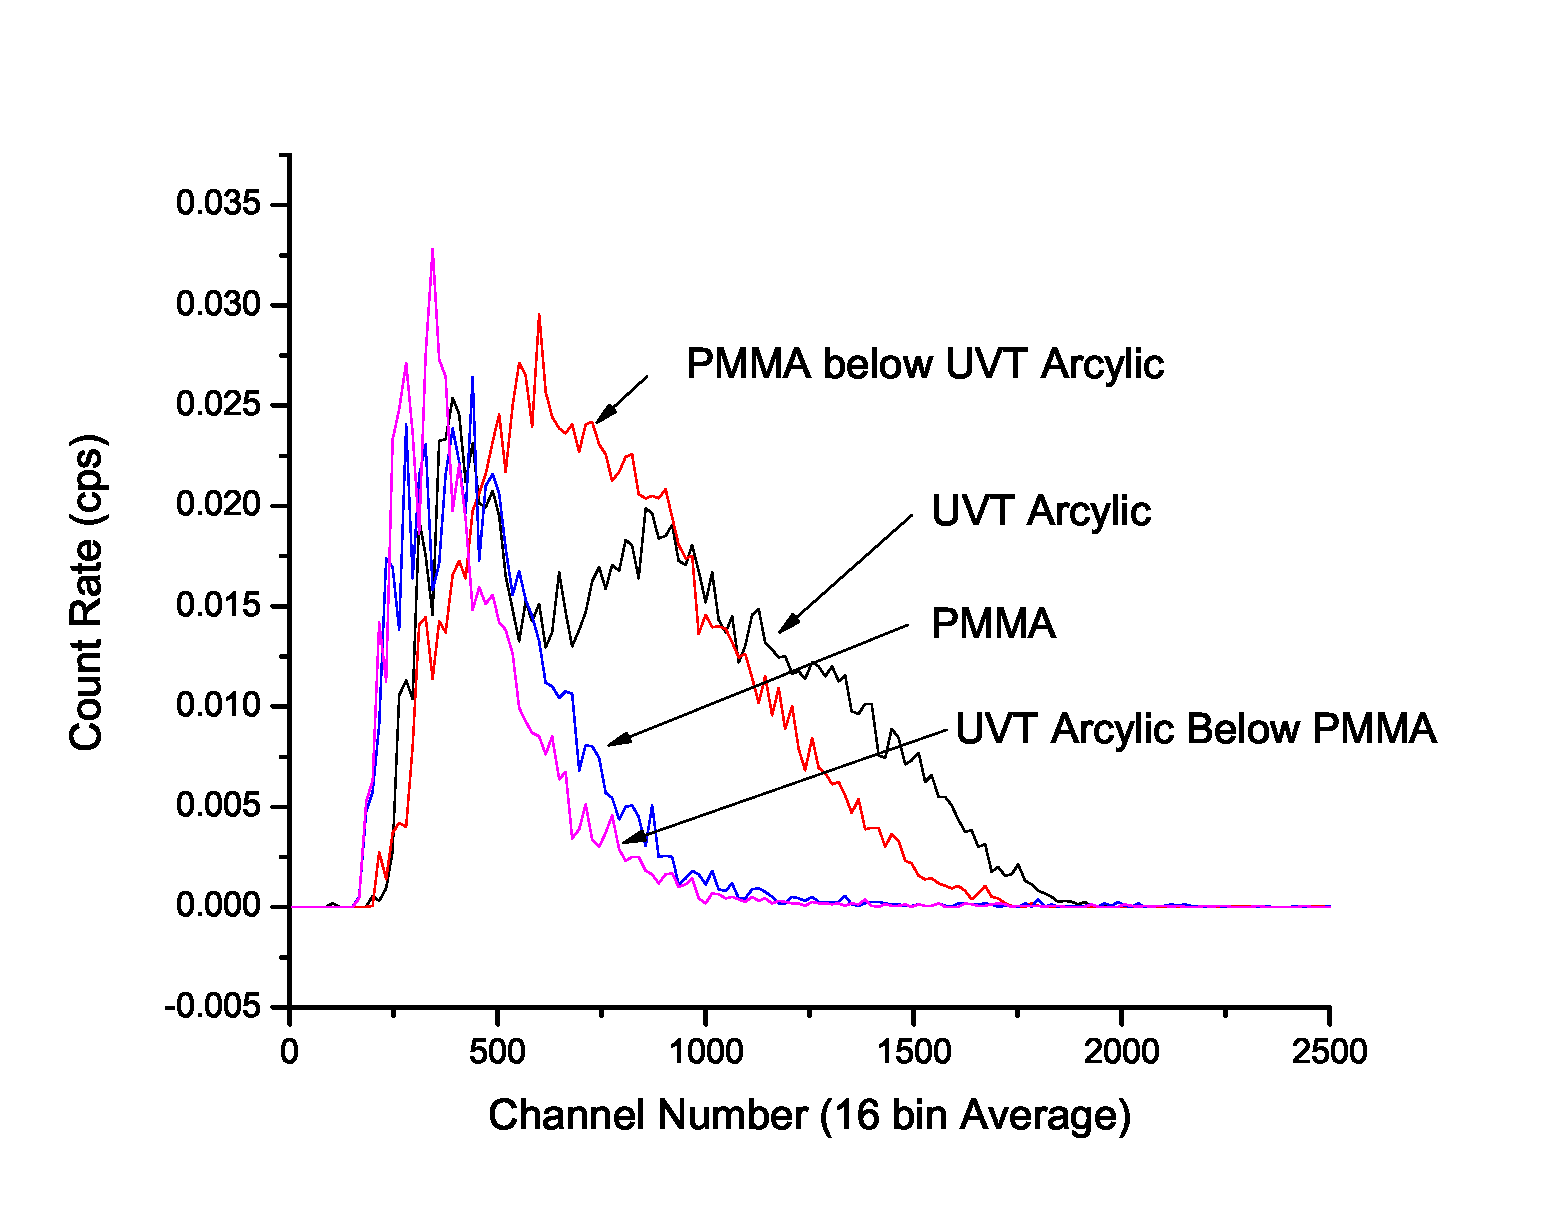
\includegraphics[width=0.7\textwidth]{UVTPMMA_LightYield}
  \caption[Measured Effect of UVT acrylic and PMMA]{Measured Neutron Spectra of UVT Acrylic and PMMA Films. It is observed that the performance of the PMMA film is not enhanced by placing it atop of a UVT acrylic disc, and the performance of a film cast on a UVT acrylic is not significantly degraded up the placing it on PMMA disc. It is noted that some performance degradation is observed, but it not clear that this is below the effects of adding a additional layer of optical coupling.}
  \label{fig:RadMeasuredExper}
\end{figure}
The measured spectra of the five fabricated films are shown in \autoref{fig:CompAm241} and \autoref{fig:CompCl36} for the alpha and beta responses.
It is observed that the \SI{6}{\mm} UVT PMMA has the lowest alpha response, while the \SI{1}{\mm} PMMA is also slightly lower than the \SI{3}{\mm} samples.
The reponse to a \iso{36}[Cl] source shows a slightly differnet trend, with the \SI{1}{\mm} PMMA film having the lowest light output, followed by the \SI{6}{\mm} UVT acryclic and finally the three \SI{3}{\mm} UVT acrylic.
\begin{figure}[ht]
  \centering
  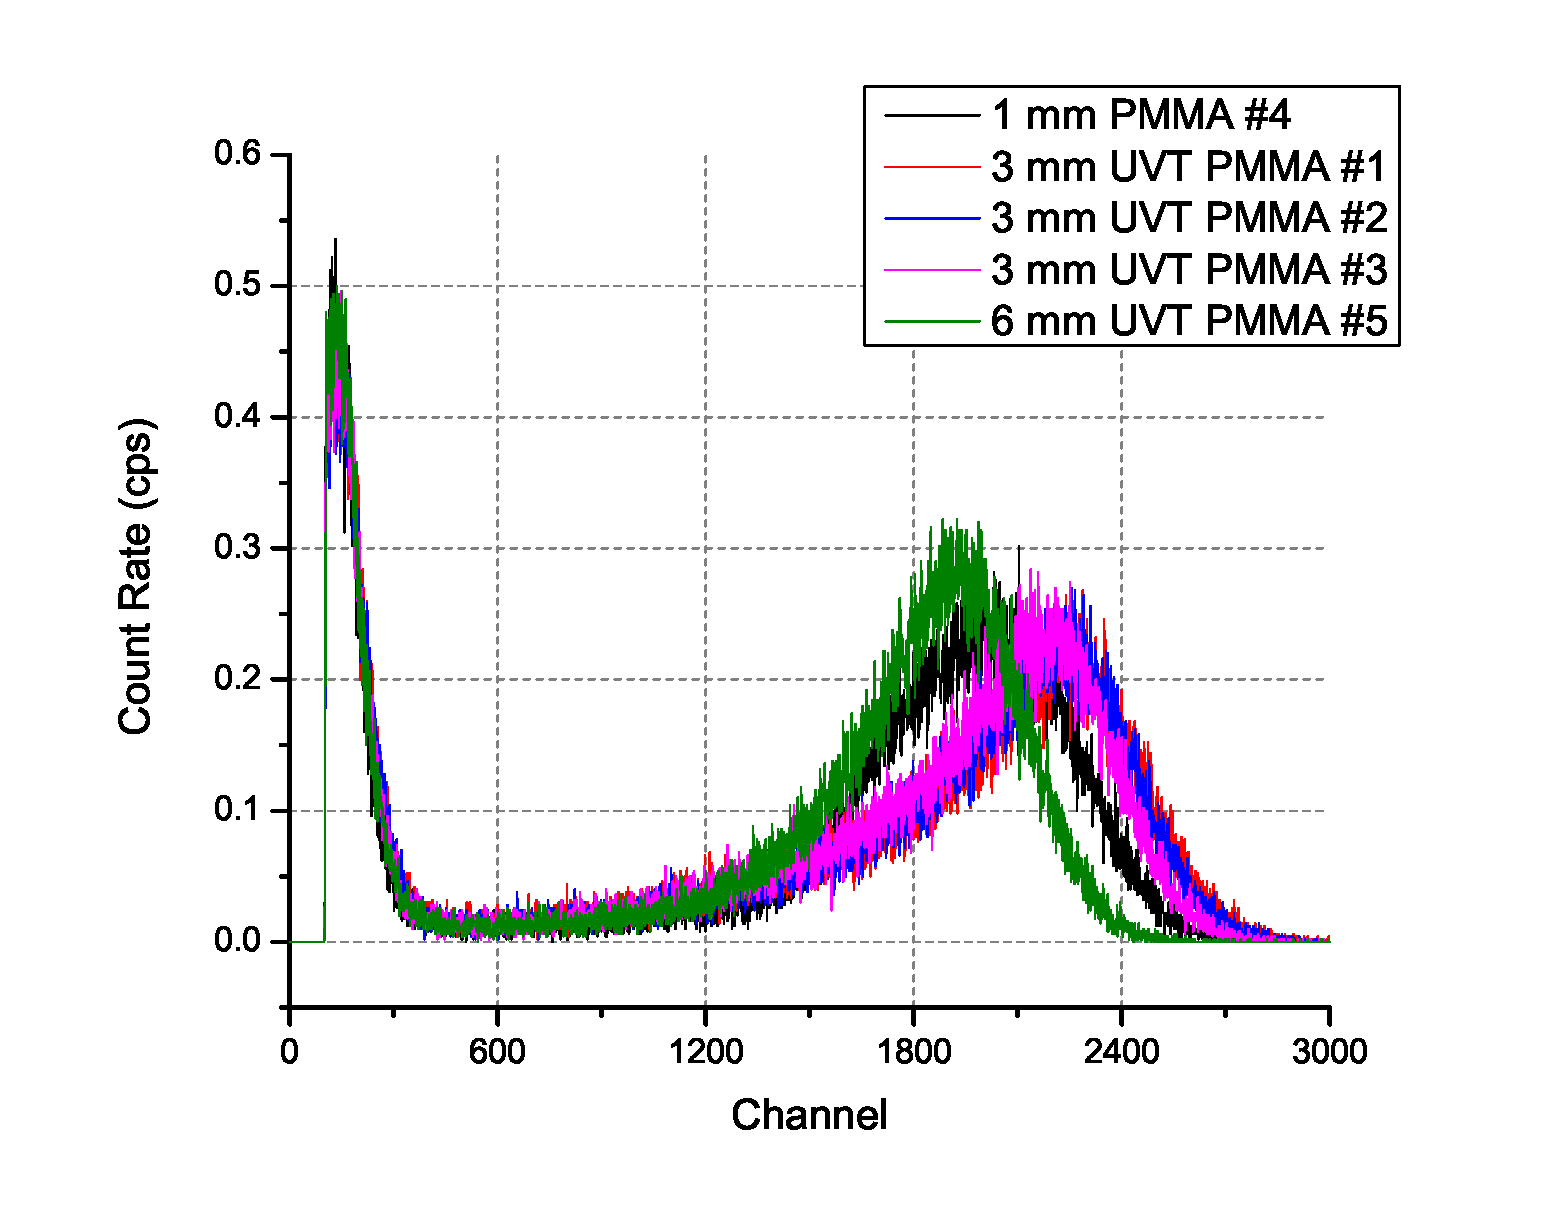
\includegraphics[width=0.7\textwidth]{50umTrials_Am241}
  \caption[Fabricated Film Comparison (Alpha)]{Comparison of the \iso[241]{Am} response of the fabricated films}
  \label{fig:CompAm241}
\end{figure}
\begin{figure}[ht]
  \centering
  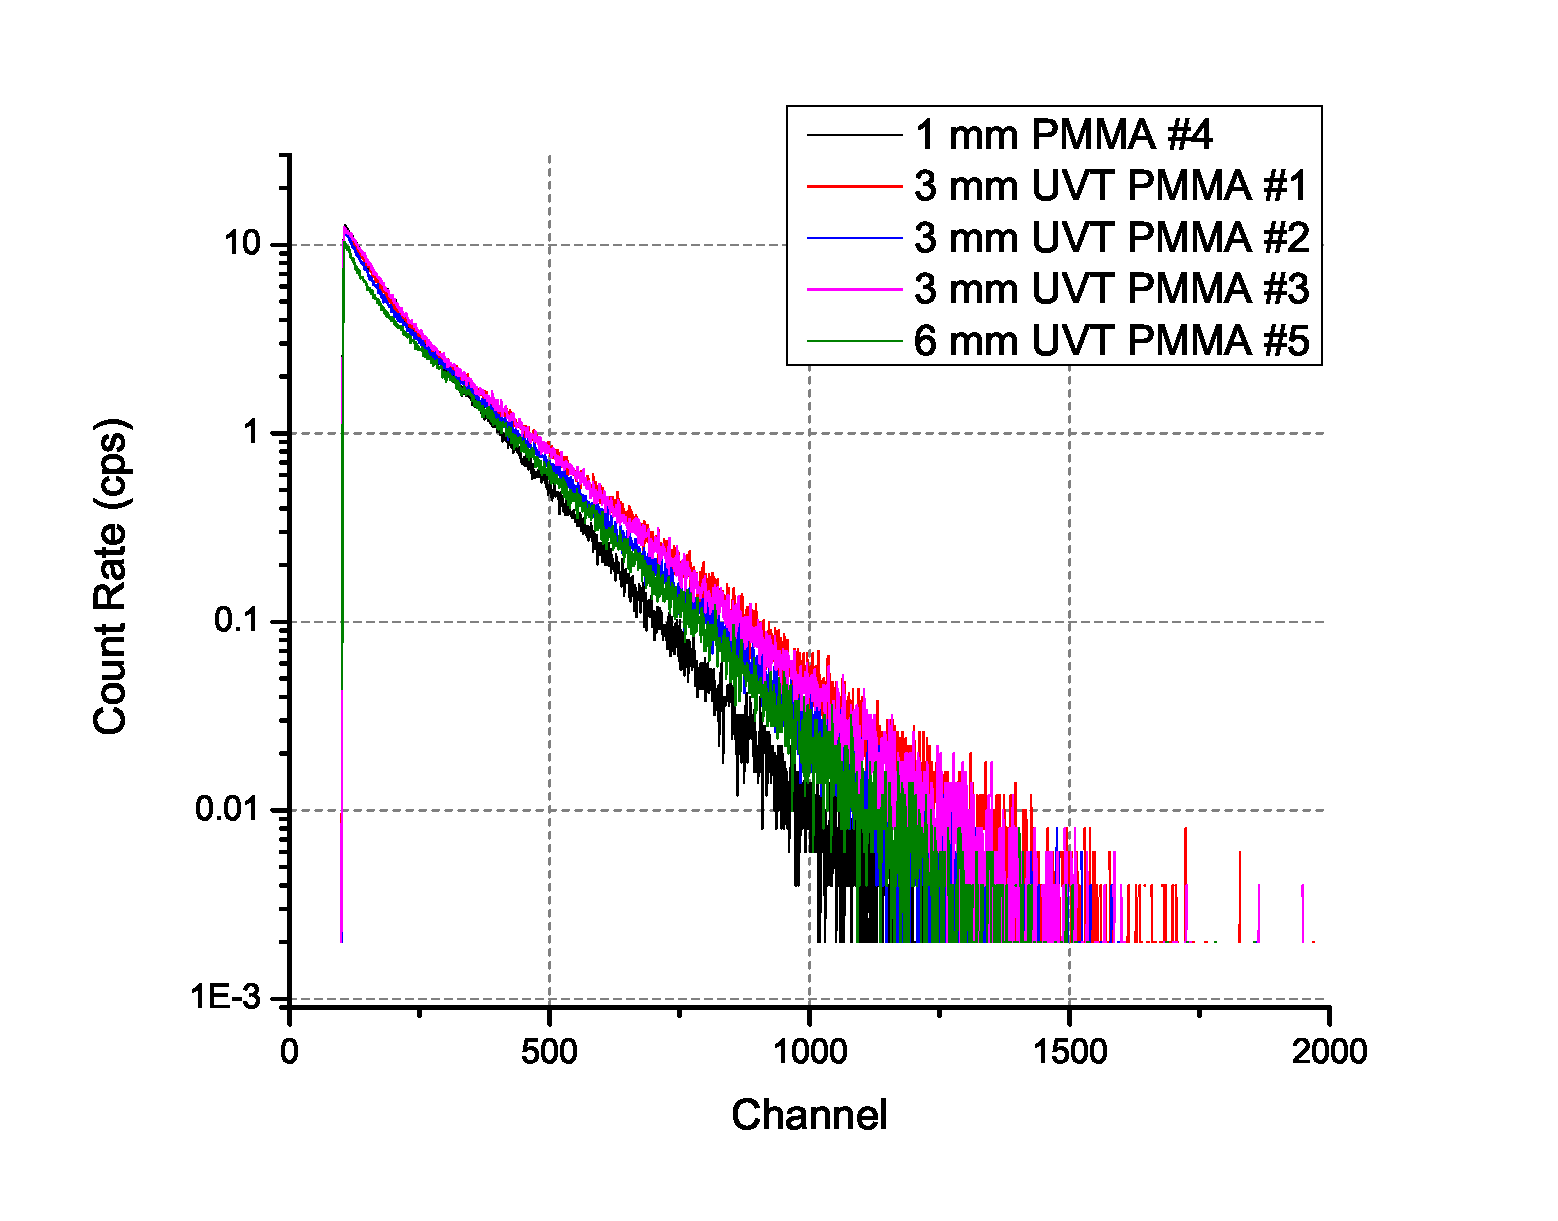
\includegraphics[width=0.7\textwidth]{50umTrials_Cl36}
  \caption[Fabricated Film Comparison (Beta)]{Comparison of the \iso[36]{Cl} response of the fabricated films}
  \label{fig:CompCl36}
\end{figure}
The gamma response of the five measured PS films is shown in \autoref{fig:CompCo60}.
It is observed that all of the films have a very similar response\footnote{It is the opinion of the author is that the gamma spectra is not an accurate assement of the performance of a film due to the lower probability of energy deposition in the film.}
The neutron spectra, \autoref{fig:CompCf252}, shows the the \SI{1}{\mm} PMMA has a dramatically different neutron response than the other films in the series.
This measurment is repeatable (\autoref{sec:MeasRepeat}) while only one is shown.
The \SI{3}{\mm} UVT PMMA films all follow the same trends; their spectra look almost identical.
Finally, the \SI{6}{\mm} UVT PMMA also has a noticable two peak spectra shape with the first peak around 250 channels and the second around 1000 channels.
\begin{figure}[ht]
  \centering
  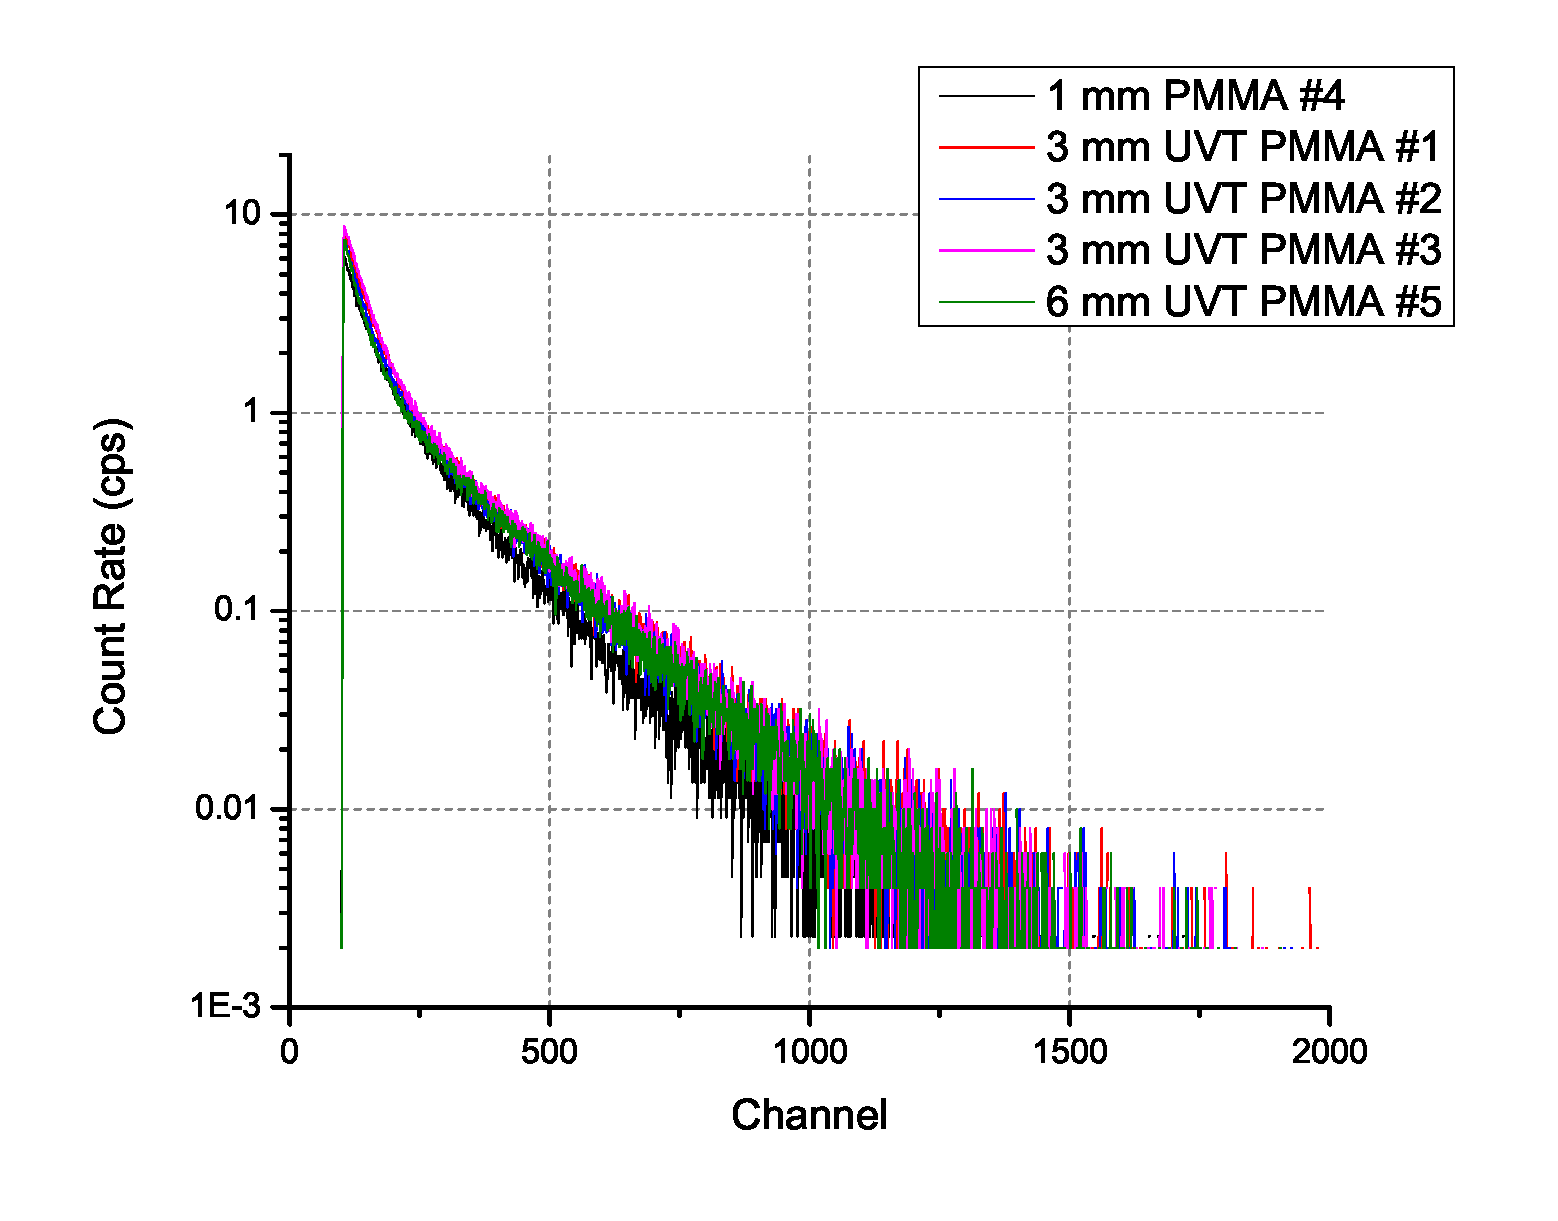
\includegraphics[width=0.7\textwidth]{50umTrials_Co60}
  \caption[Fabricated Film Comparison (Gamma)]{Comparison of the \iso[60]C{Co}response of the fabricated films}
  \label{fig:CompCo60}
\end{figure}
\begin{figure}[ht]
  \centering
  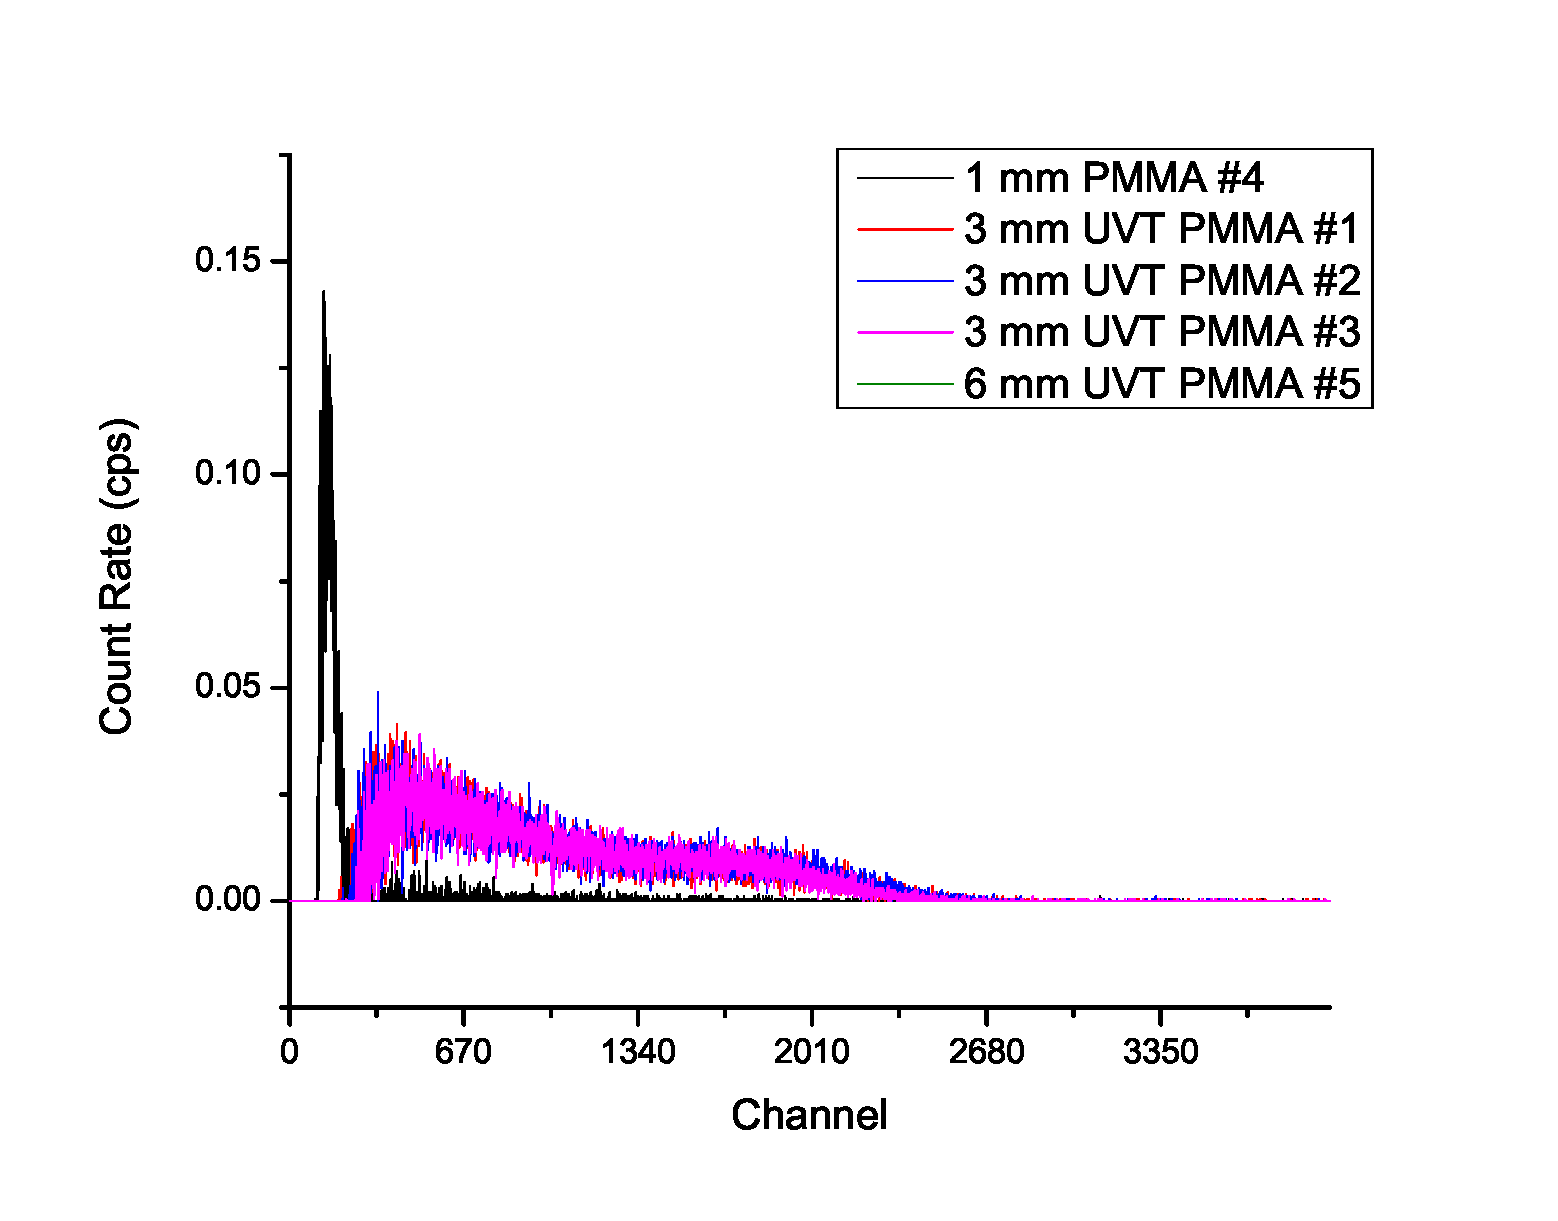
\includegraphics[width=0.7\textwidth]{50umTrials_CfNet}
  \caption[Fabricated Film Comparison (Neutron)]{Comparison of the \iso[252]{Cf} response of the fabricated films. It is evident that the PMMA film (Sample 4) has a much lower neutron response in addition to a differnet spectral shape than the other samples.}
  \label{fig:CompCf252}
\end{figure}
\section{Conclusions}
It is evident that the neutron performance of the \SI{1}{\mm} PMMA film has a much lower light output than the films mounted on UVT PMMA, while the light yeild (as determined by an \iso{241}[Am] and \iso{36}[Cl]) of the \SI{1}{\mm} PMMA is only slightly lower than the UVT acrylic films.
An intresting feature that is evident in the UVT acrylic films is a peak, slight trough, and then another shallow peak.
It is thought that the first peak is due to the energy deposition of the alpha (range \SI{10}{\um} in PS, \SI{2.05}{\MeV}) while the full energy deposition (adding in the triton of range \SI{62}{\um} and \SI{2.78}{\MeV}) occurs at the higher peak.
As the films are only \SI{50}{\um} thick it is highly probable that the alpha does not deposit all of it's energy in the film.

It is unclear why the \SI{1}{\mm} PMMA has a completly differnet neutron spectral shape.
Attenuation of light in the disc would be expected to impact all of the light yields equally, and a dramatic decrease is the light yield is not observed.
The repeatable low energy neutron peak suggests that complete energy deposition from the alpha is occuring, while the triton is not depositing any of its energy.
A possibe cause of this might be the disc chemically interacting with the cast film, causing the film to be effectively thinner than designed.

The following films, \autoref{tab:1MMPMMAFilms}, are cast upon a \SI{1}{\mm} PMMA disc, and as shown above their neutron performance measurment is suspect.
\ctable[cap={\SI{1}{\mm} PMMA Films},caption={Film cast on \SI{1}{\mm} PMMA Disc. The neutron performance of these films should be revied.},label={tab:1MMPMMAFilms},]{l | l}{\tnote[$\dagger$]{Supporting spectra not found}}{%
\FL
Film Name & Date Manufactured \\
\midrule
\path{PS_LiF(20.0)_POP(5.29)_25um_7Jun12} & \printdate{7/6/2012} \tmark[$\dagger$] \\
\path{PS_LiF(20.3)_POP(4.62)_25um_29May12 Annealed} & \printdate{29/5/2012}  \\
\path{PS_LiF(30.0)_POP(4.64)_25um_29May12 Annealed} & \printdate{29/5/2012}  \\
\path{PS_LiF(20.1)_POP(5.12)_50um_29May12} & \printdate{29/5/2012} \tmark[$\dagger$] \\
\path{PS_LiF(10)_POP(5)_50um_28Feb13} & \printdate{28/2/2013} \tmark[$\dagger$] \\
\path{PS_LiF-n(10)_POP(5)_50um_28Feb13} & \printdate{28/2/2013} \tmark[$\dagger$] \\
\LL}
It is recomended not to use the \SI{1}{\mm} PMMA disc for neutron performance measruments.
\pagebreak
\appendices
\section{Measurment Repeatiblity}
\label{sec:MeasRepeat}
The conlusion that PMMA disc has a signifantly lower neutron performance is supported by two measurments of the single prepared film.
The order of the measurments was Trial 1, then Sample 3, and then returning to Trial 1 once it was noticed that it deviated largely from Sample 3.
It is observed in \autoref{fig:MeasRepeatLY} that Trial 2 samples tend to have a higher light yield. 
This may be due to a slight temperate based changed in the electronic gains, or simply due to better coupling and light collection in Trial 2 comapred to Trial 1.
However, the increase in light output is not observed in the gamma spectra, so if better coupling is the cause of the increased light output it would be expected that all of the Trial 2 data would be higher by the same amount.
The neutron spectra (\autoref{fig:MeasRepeatNeutron}) show excellent repeatibility, and both spectra have the skewed shape.
\begin{figure}
  \centering
  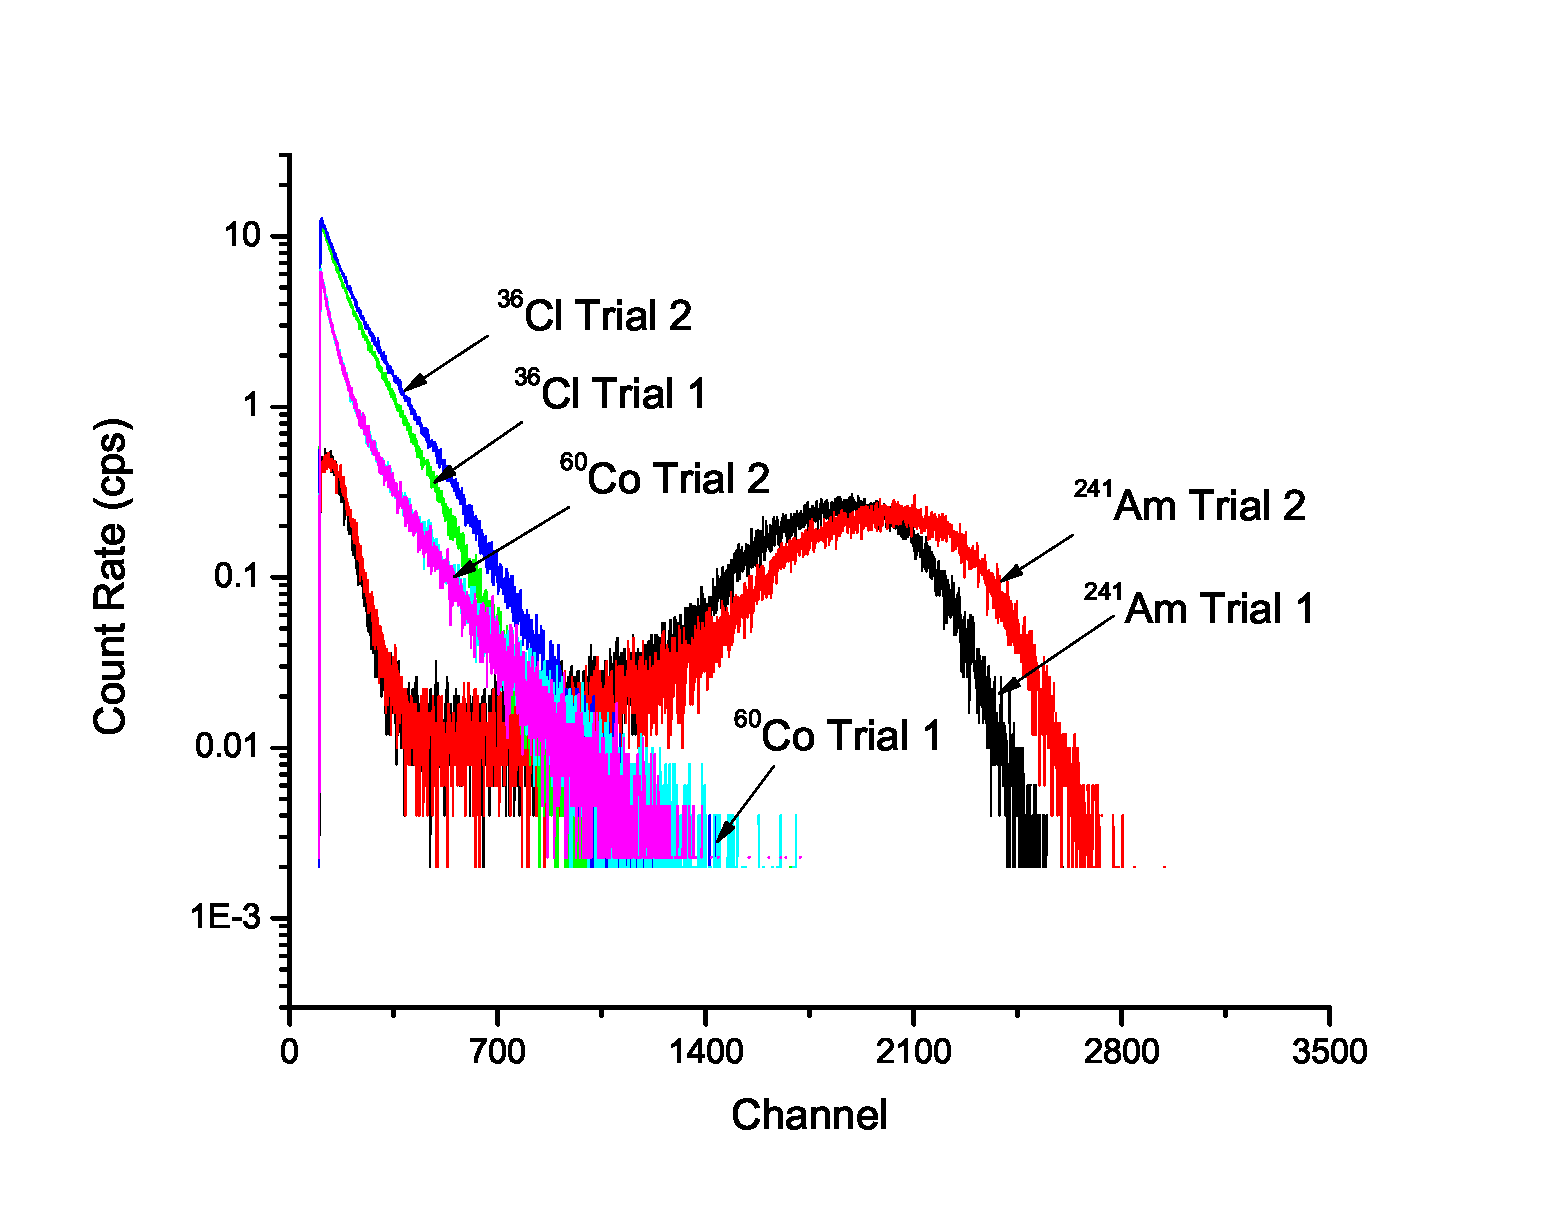
\includegraphics[width=0.7\textwidth]{50umTrials_PMMARepeat}
  \caption[PMMA Light Yield Repeatiblity]{Repeatiblity of the light yield measurments of the \SI{1}{\mm} PMMA disc. It is observed that the alpha and beta light yield in Trial 2 is higher than Trial 1, while the gammas are essentially overlapping.}
  \label{fig:MeasRepeatLY}
\end{figure}
\begin{figure}
  \centering
  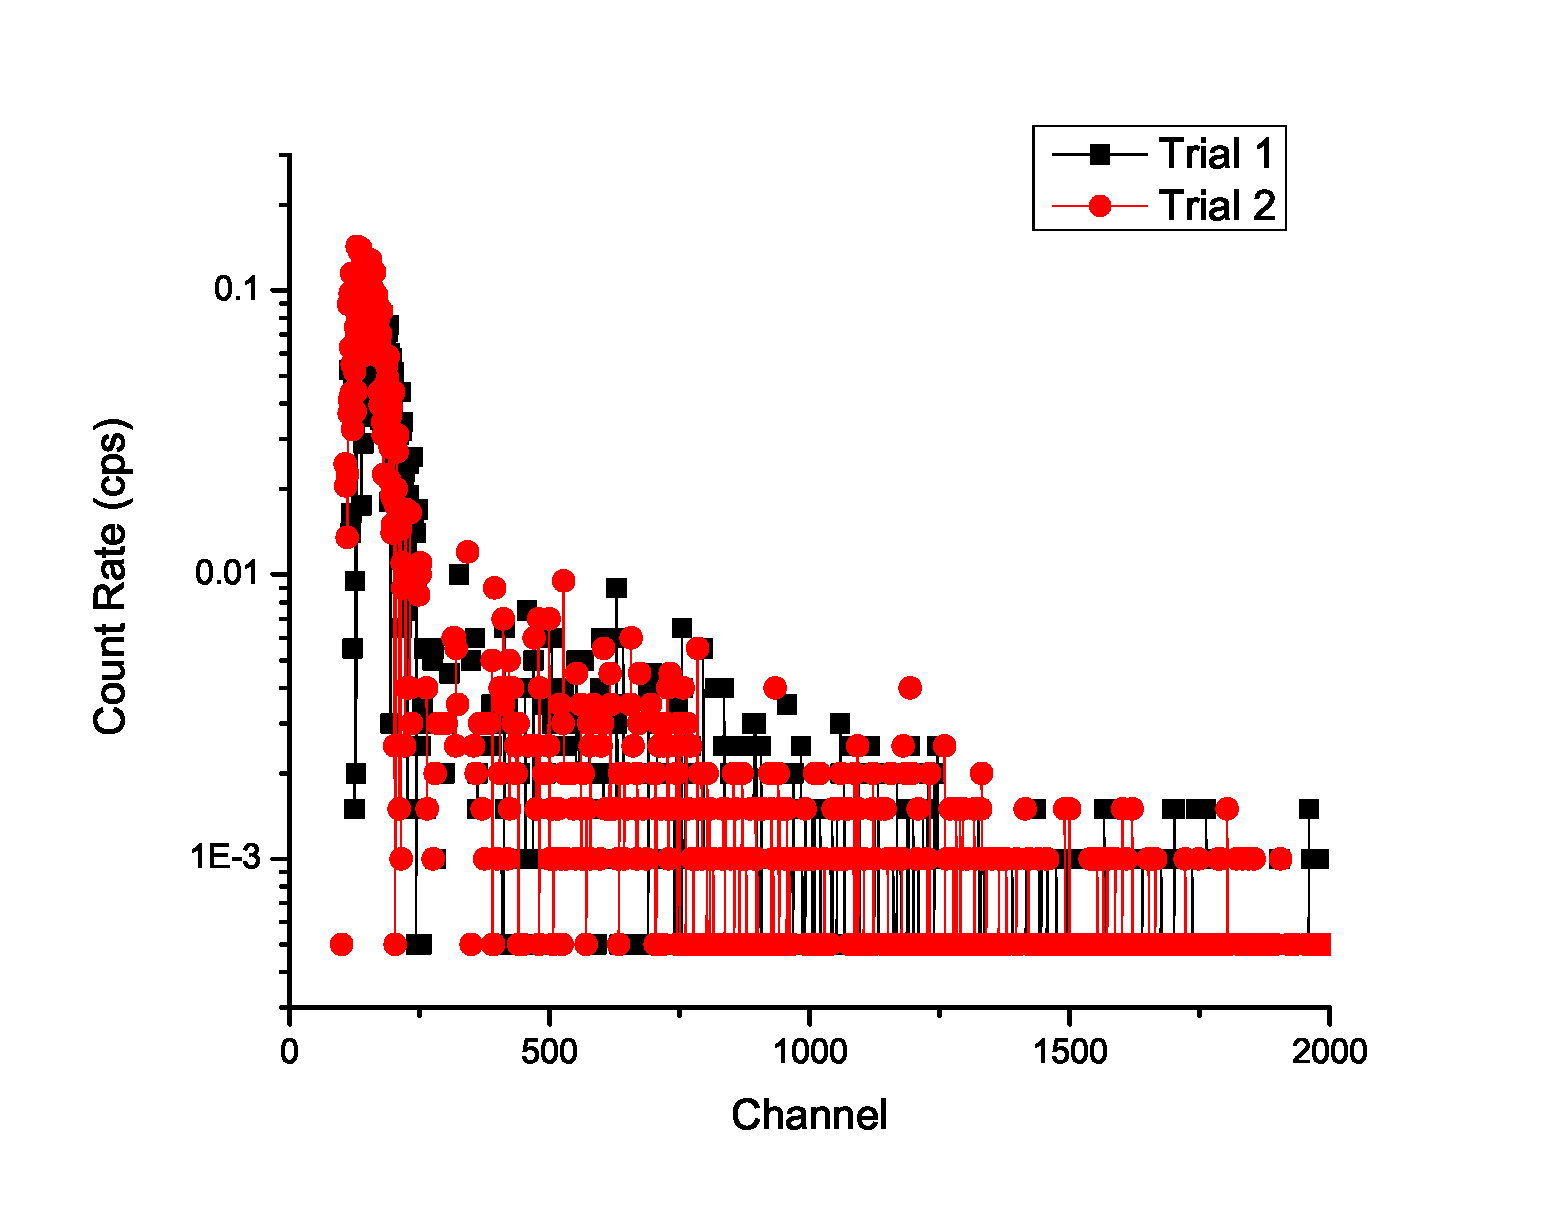
\includegraphics[width=0.7\textwidth]{50umTrials_PMMARepeat_Cf252}
  \caption[PMMA Neutron Repeatiblity]{Repeatiblity of the neutron measurments of the \SI{1}{\mm} PMMA disc. It is observed that both of the measured spectra have the strange shape.}
  \label{fig:MeasRepeatNeutron}
\end{figure}

\section{File Locations and Report Status}
The spectra files for this report may be found in \path{SpectraFiles/(0)_2013_Data/PSArcylicUVT_vs_PMMA}, and the plots were generated with the OriginPro project \path{AcrylicUVT.opj}.
This document is may be found in \LaTeX format at \url{\svnkw{HeadURL}}.  
The latest revision for this file is \svnrev, and was on \svndate, committed by \svnauthor.
The films were fabricated by Andrew Mabe.
\end{document}
